\documentclass[12pt,a4paper]{article}

% --- Essential Packages ---
\usepackage[utf8]{inputenc}
\usepackage{geometry}
\geometry{a4paper, margin=1in}
\usepackage{amsmath}
\usepackage{graphicx}
\usepackage{hyperref}
\usepackage{subcaption}
\usepackage{float}

% --- Hyperlink Colors ---
\hypersetup{
    colorlinks=true,
    linkcolor=blue,
    urlcolor=cyan
}

% --- Title Page Info ---
\title{
     \vspace*{1cm}
    
\includegraphics[width=6cm]{assets/logo.png} \\
    \vspace*{1cm}
    \large Brno University of Technology \\
    \large Faculty of Information Technology \\
    \vspace{2cm}

    \textbf{Analysis of Transport Protocols (TCP/QUIC) in Extreme Network Environments} \\
    \vspace*{1cm}
    \large Project Report\\
    \vspace{1cm}
    \large{PDSe 25/26} \\
    \vspace{1cm}
    \vspace*{1cm}
    \large Eyobed Awel Nuri\\
    \large xnuriey00 \\
    \vfill
    \date{\today}
}


\begin{document}

\maketitle
\newpage

\tableofcontents
\newpage

% --- Main Content ---


\section{Introduction}
In the OSI model of networking, the transport layer is responsible for providing process to process communication using a logical connection. It sits between the application layer and the network layer.
This is achieved by using dedicated port numbers for each application running on the host. Additionally, the transport layer implements segmentation, flow control and congestion control. The latter is the main focus of this project, in which we explore the performance of different algorithms used for congestion control.

\subsection{Transport Protocols}
The transport layer defines the services conceptually and various specific protocols handle the actual implementation. Different protocols provide services appropriate to particular application scenarios. Transport protocols are broadly classified into two categories: connection-oriented and connectionless.

Connection-oriented protocols, such as TCP, establish a logical connection through a handshake before data transmission begins. This means we have reliability, packet ordering, and flow control, at the cost of some overhead. Connectionless protocols, like UDP, transmit data without a setup, offering lower latency and overhead but no guarantees for delivery.

In this report we review two connection-oriented protocols, TCP and QUIC. 



\subsubsection{Transmission Control Protocol (TCP)}
TCP is a connection-oriented protocol that defines connection establishment, data transfer, and connection termination. To understand TCP, it is useful to discuss the TCP packet itself first, as shown in Figure \ref{fig:tcp_header}.

\begin{figure}[ht]
    \centering
    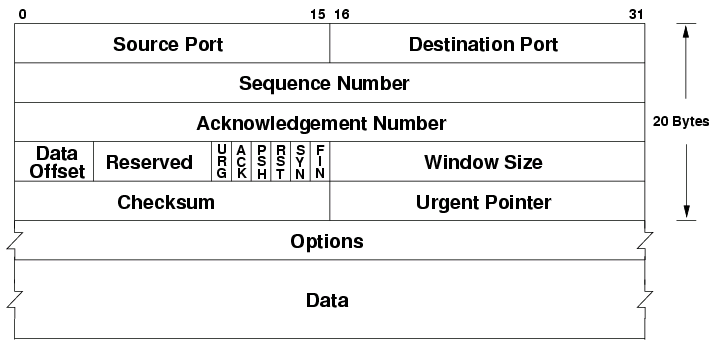
\includegraphics[width=0.8\textwidth]{assets/TCP_header.png}
    \caption{TCP Protocol Header \cite{kovako2011}}
    \label{fig:tcp_header}
\end{figure}

The TCP header is usually 20 bytes long (up to 60 bytes with options) and contains several fields:
\begin{itemize}
    \item \textbf{Source and Destination Ports:} 16-bit fields used to identify applications
    \item \textbf{Sequence Number:} A 32-bit field for reassembly in the correct order.
    \item \textbf{Acknowledgment Number:} A 32-bit field used to confirm reception of data and indicate the next expected byte.
    \item \textbf{Data Offset:} A 4-bit field that indicate where the data begins.
    \item \textbf{Control Flags:} Includes bits such as \texttt{SYN}  for connection establishment, \texttt{ACK}  for valid acknowledgment numbers, and \texttt{FIN}  for terminating the connection.
    \item \textbf{Window Size:} A 16-bit field used for flow control, specifying the number of bytes the receiver is able to recieve.
    \item \textbf{Checksum:} A 16-bit field used for error-checking.
    \item \textbf{Urgent Pointer:} A 16-bit field that points to the end of urgent data.
    \item \textbf{Options:} Additional functionality
    \item \textbf{Data:} The actual information being transmitted following the header.
\end{itemize}

\paragraph{Connection Establishment}
TCP uses a 3-way handshake to establish a reliable connection between a client and a server:
\begin{enumerate}
    \item \textbf{SYN:} The client sends a segment with the \texttt{SYN} flag set and an initial sequence number ($x$).
    \item \textbf{SYN-ACK:} The server responds with both \texttt{SYN} and \texttt{ACK} flags set, acknowledging the client's sequence number ($x+1$) and providing its own initial sequence number ($y$).
    \item \textbf{ACK:} The client sends an \texttt{ACK} segment acknowledging the server's sequence number ($y+1$), completing the handshake.
\end{enumerate}

\begin{figure}[H]
    \centering
    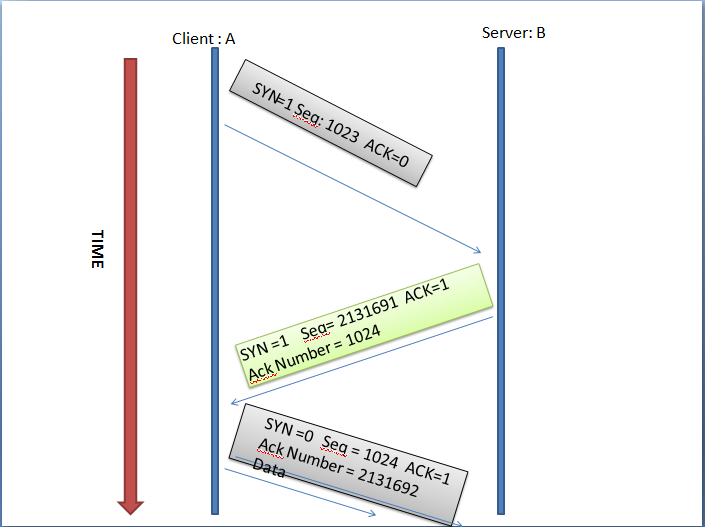
\includegraphics[width=0.8\textwidth]{assets/TCP_Handshake.png}
    \caption{TCP Three-Way Handshake \cite{sajidur2013}}
    \label{fig:tcp_handshake}
\end{figure}


\paragraph{Data Transfer and Error Control}
Once established, data is partitioned into segments, the size of which is determined by the \textbf{Maximum Segment Size (MSS)} negotiated during the handshake. Then TCP utilizes a Sliding Window mechanism for data transfer and flow control. This allows the sender to transmit multiple segments before requiring an acknowledgment, up to the limit specified by the receiver's window size. Reliability is guaranteed through error detection (checksums) and error recovery; if segments arrive out of order, they are buffered until the missing data is retransmitted and received. TCP uses cumulative acknowledgments, where an ACK for sequence number $n$ implies that all bytes up to $n-1$ have been successfully received. This is important difference between TCP and the other protocol QUIC.

\paragraph{Connection Termination}
 follows a four-way handshake, allowing each side to close its side independently:
\begin{enumerate}
    \item \textbf{FIN:} One host sends a \texttt{FIN} segment to indicate it has finished sending.
    \item \textbf{ACK:} The other host acknowledges the \texttt{FIN} and may continue to send its remaining data.
    \item \textbf{FIN:} Once the second host is finished, it sends its own \texttt{FIN} segment.
    \item \textbf{ACK:} The first host sends a final \texttt{ACK}, and the connection is closed after a timeout.
\end{enumerate}

\begin{figure}[H]
    \centering
    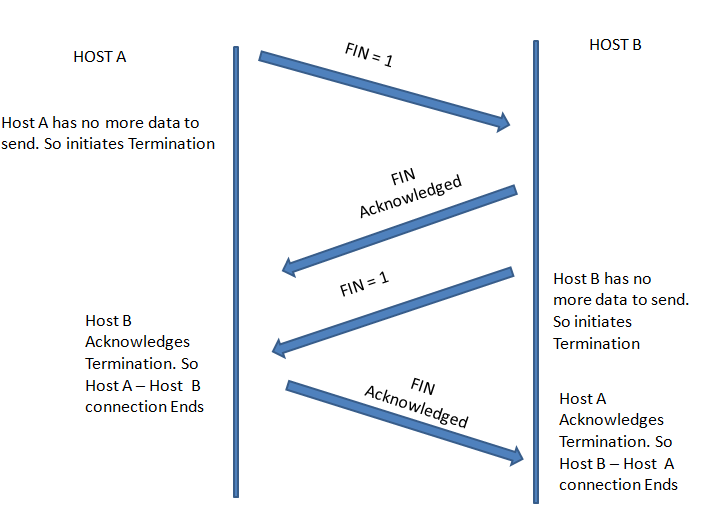
\includegraphics[width=0.8\textwidth]{assets/TCP_connection_Termination.png}
    \caption{TCP Four-Way Termination  \cite{sajidur2013term}}
    \label{fig:tcp_termination}
\end{figure}

\paragraph{TCP States}
a TCP connection transitions through several states defined by the TCP State Machine \cite[p.~756]{forouzan2013}. These states include:
\begin{itemize}
    \item \texttt{LISTEN:} The server is waiting for an incoming connection request.
    \item \texttt{SYN-SENT / SYN-RECEIVED:} The  states during the three-way handshake.
    \item \texttt{ESTABLISHED:} The state where data can be exchanged.
    \item \texttt{FIN-WAIT / CLOSE-WAIT / LAST-ACK:} States involved in the termination of the connection.
    \item \texttt{TIME-WAIT:} A final state where the host waits to be sure the remote host received the final ACK, this prevent delayed packets from interfering with future connections.
\end{itemize}


\subsection{Network Congestion} \label{subsec:congestion_control}

\paragraph{Congestion}
Flow control mechanisms make sure that the receive window is never overflowed with bytes However, intermediate routers handling data from multiple senders can become overwhelmed and lose segments. This  forces the transport protocol to retransmit lost segments, worsening the congestion. Therefore, while flow control protects the receiver, congestion control protects the entire network path. \cite{forouzan2013},

\paragraph{Principles of Congestion Avoidance}
Since transport protocols cannot aggressively insert segments without damaging the network, nor be too careful and waste bandwidth, they must have some policies to accelerate transmission when the network is clear and decelerate when congestion is detected. To accomplish this, protocols set  transmission rate using a dedicated state variable known as the \textit{Congestion Window} (\texttt{cwnd}). the actual volume of unacknowledged data a sender can insert into the network is  governed by the \textit{Send Window}, $\text{Send Window} = \min(\texttt{cwnd}, \texttt{rwnd})$ \cite[p.~777]{forouzan2013}.

Algorithms set the size of the cwnd based on detection of packet loss(Reno and CUBIC) or modeling the bandwidth(BBR).
\subsubsection{Congestion Control in TCP}
In TCP, the receiver's \texttt{rwnd}  is continuously sent back to the sender via the Window Size field in its  header. so to set \texttt{cwnd}, TCP relies on a  feedback  from the other end to detect congestion: ACKs \cite[p.~778]{forouzan2013}. It categorizes congestion into two levels:
\begin{itemize}
    \item \textbf{Strong Congestion (Time-out):} indicating severe packet loss in the network.
    \item \textbf{Weak Congestion (Three Duplicate ACKs):} indicating the network is only slightly congested or has already recovered.
\end{itemize}

For regulating the \texttt{cwnd} TCP uses several algorithms:
\begin{itemize}
    \item \textbf{TCP Reno:} 
    \begin{itemize}
        \item \textbf{Slow Start:} The sender begins with $\texttt{cwnd} = 1$ MSS. For every ACK received, the window is incremented by one MSS,  doubling the window each RTT . A separate state variable, \texttt{ssthresh}, is initialised to a high value. This probing continues until \texttt{cwnd} reaches \texttt{ssthresh}, at which point the algorithm transitions to Congestion Avoidance.

        \item \textbf{Congestion Avoidance:} The sender now grows the window linearly, incrementing \texttt{cwnd} by approximately 1 MSS per RTT (i.e., $cwnd = cwnd + \frac{MSS \times MSS}{cwnd}$per ACK). This  continues until a congestion is detected.

        \item \textbf{Congestion Detection and Response:}  Reno distinguishes two severity levels \cite[p.~783]{forouzan2013}:
        \begin{itemize}
            \item \textbf{Fast Retransmit \& Fast Recovery (3 Duplicate ACKs):} Weak congestion. Reno immediately Fast Retransmit. It then enters Fast Recovery: 
            \begin{align*}
                \texttt{ssthresh} &= \frac{\texttt{cwnd}}{2} \\
                \texttt{cwnd}     &= \texttt{ssthresh} + 3 \text{ MSS}
            \end{align*}
            While waiting for acknowledgement of the retransmitted segment, each additional duplicate ACK indicates another packet buffered at the receiver, so the window is further added.
            \[ \texttt{cwnd} = \texttt{cwnd} + 1 \text{ MSS} \]
            Once a new ACK confirms recovery, the window back to the threshold before resuming Congestion Avoidance:
            \[ \texttt{cwnd} = \texttt{ssthresh} \]

            \item \textbf{Timeout :} Strong Congestion.the threshold is halved and the window is reset to 1 MSS,  a restart of Slow Start:
            \begin{align*}
                \texttt{ssthresh} &= \frac{\texttt{cwnd}}{2} \\
                \texttt{cwnd}     &= 1 \text{ MSS}
            \end{align*}
        \end{itemize}
    \end{itemize}
Reno is  \textbf{loss-based} nature: it treats any packet drop as  evidence of congestion, regardless of the actual cause. This makes it  vulnerable to environments with  random packet loss.

\begin{figure}[H]
    \centering
    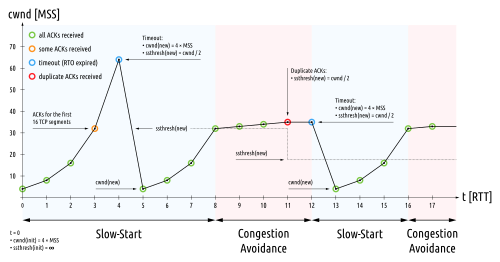
\includegraphics[width=0.8\textwidth]{assets/reno.png}
    \caption{TCP Slow-Start and Congestion Avoidance (Reno) \cite{fleshgrinder2014}}
    \label{fig:reno_cwnd}
\end{figure}


    \item \textbf{TCP CUBIC:} The TCP CUBIC is designed to address the short coming of reno on long RTT network. In CUBIC the \texttt{cwnd} is not based on RTT, it is based on the host's time and is calculated using the following formula:
    \[
        W(t) = C(t - K)^3 + W_{\max}
    \]
    where $W_{\max}$ is the window size at the point of the last packet loss, $t$ is the elapsed time since that loss, $C$ is a scaling constant, and $K$ is the time the function takes to grow back to $W_{\max}$ from its reduced value.\cite{ha2008cubic, rfc9438cubic} This cubic curve has three phases:
    \begin{itemize}
        \item \textbf{Concave (below $W_{\max}$):} the value of $(t-K)$ is negative
        \item \textbf{Plateau (near $W_{\max}$):} $(t-K)^3$ term approaches zero
        \item \textbf{Convex (above $W_{\max}$):} the cubed term becomes positive and grows exponentially
    \end{itemize}
    Upon detecting a loss (via 3 DUP ACKs or timeout), CUBIC performs a multiplicative decrease to $\beta_{\text{cubic}} \approx 0.7$ of the current window and records the new $W_{\max}$ \cite{ha2008cubic}. Like Reno, CUBIC is also a loss-based algorithm.

    \item \textbf{TCP BBR (Bottleneck Bandwidth and RTT):} Developed at Google in 2016, BBR uses network model instead of loss based one \cite{cardwell2016bbr}. While Reno and CUBIC react to network congestion, BBR attempts to {model} the network and {prevent} congestion before it begins. It uses two physical parameters:
    \begin{itemize}
        \item $BtlBw$: the bottleneck bandwidth, the minimum available throughput along the entire path.
        \item $RTprop$: round-trip propagation time, the minimum RTT seen with no load
    \end{itemize}
From these two variables, BBR calculates the Bandwidth-Delay Product (BDP):$$BDP = BtlBw \times RTprop$$

    BBR continuously updates its network model by cycling through four distinct states:
    \begin{itemize}
        \item \textbf{STARTUP:} Probes capacity by exponentially increasing the sending rate until $BtlBw$ plateaus
        \item \textbf{DRAIN:} Briefly lowers the pacing rate to empty any queues accumulated during STARTUP
        \item \textbf{PROBE\_BW:} The steady-state cycle
        \item \textbf{PROBE\_RTT:} If a new minimum RTT is not seen for 10 seconds, BBR  reduces its \texttt{cwnd} to 4 MSS to clear all queues and measure $RTprop$ \cite{cardwell2023bbr}.
    \end{itemize}
    BBR is  immune to random  interference that harm loss-based algorithms like Reno and CUBIC.
\end{itemize}

\section{Methodology}

\subsection{Network Topology}

\textbf{Linux Namespaces}
The laboratory was built using Linux Network Namespaces. Three namespaces were created : \texttt{client}, \texttt{router}, and \texttt{server} interconnected by two virtual Ethernet (\texttt{veth}) pairs:

\begin{center}
\texttt{client (c\_eth)} $\longleftrightarrow$ \texttt{(r\_in) router (r\_out)} $\longleftrightarrow$ \texttt{(s\_eth) server}
\end{center}

A script (\texttt{setup.sh}) is developed that builds and if neccessary rebuilds the topology from scratch if it is in reproduction enviroment.\\
\textbf{Namespace and Link Creation.} The script creates the three required namespaces and maps virtual ethernet pairs (\texttt{veth}) between them:

\begin{verbatim}
# Creating namespaces: client, router, server
sudo ip netns add client
sudo ip netns add router
sudo ip netns add server

# Create and assign virtual ethernet cable 
sudo ip link add c_eth type veth peer name r_in
sudo ip link set c_eth netns client
sudo ip link set r_in netns router
\end{verbatim}

\textbf{IP Addresses.}  Once the virtual cables are connected,IP addresses inside subnets (\texttt{10.0.0.0/24} and \texttt{10.0.1.0/24}) are established:

\begin{verbatim}
# Bind static IP addresses to the interfaces
sudo ip netns exec client ip addr add 10.0.0.1/24 dev c_eth
sudo ip netns exec router ip addr add 10.0.0.2/24 dev r_in
\end{verbatim}

\textbf{Forwarding and Routing.} Finally, IPv4 packet forwarding is enabled in the router namespace. 

\begin{verbatim}
# Enable IPv4 packet forwarding
sudo ip netns exec router sysctl -w net.ipv4.ip_forward=1 > /dev/null

# Establish routes
sudo ip netns exec client ip route add 10.0.1.0/24 via 10.0.0.2
\end{verbatim}

\textbf{Hardware Offload Disabling.} To avoid hardware offloading optimization from polluting the evaluation it is disabled.

\begin{verbatim}
sudo ip netns exec client ethtool -K c_eth tso off gso off gro off ...
\end{verbatim}

\textbf{Connectivity Check.} Finally, The setup is tested via a simple ping: \texttt{ping -c 3 10.0.1.1}.

This script is run once and then individual experiments are conducted with different script that changes the router environment and runs the tests as indicated in further chapters.

\subsection{Extreme Environment Simulations}

Experiments are divided by base transport protocol (e.g., \texttt{1\_TCP\_Protocol}) and  categorized into environmental profiles in the file system. Each directory acts as an individual testbed, having its own test runner script (\texttt{run\_test.sh}). This separation of concerns is beneficial as it helps us individualy rerun a particular test scenario.

When run, these scripts clean the previous enviroments. They then set the hostile conditions using Linux Traffic Control (\texttt{tc}), spawns background measurments, and executes the tests sequentially for all targeted algorithms. 

The following Traffic Control (\texttt{tc}) rule has been applied on all test scenarios to limit cpu and space usage over run:

\begin{verbatim}
   sudo ip netns exec router tc qdisc add dev r_out root handle 1: 
   htb default 10 r2q 1
   sudo ip netns exec router tc class add dev r_out parent 1: 
   classid 1:10 htb rate 100mbit
   sudo ip netns exec router tc qdisc add dev r_out parent 1:10 
   handle 10: netem delay 20ms  limit 250
\end{verbatim}

It limits the rate to 100mbps and delay to 20ms and buffer size to 250 packets to simulate a realistic normal enviroment.

The rule is then modified to simulate the following extreme enviroments:

\subsubsection{Coffee Shop Wi-Fi}
Simulating a congested public Wi-Fi access point, this profile applied a $3\%$  packet loss.

\begin{verbatim}
    sudo ip netns exec router tc qdisc add dev r_out parent 1:10 handle 10: 
    netem delay 20ms loss 3% limit 250
\end{verbatim}

\subsubsection{Starlink Satellite}
Simulating satellite broadband, this profile utilized a $600\text{ms}$  delay. To model atmospheric interference, a $50\text{ms}$ latency jitter was added.

\begin{verbatim}
   sudo ip netns exec router tc qdisc add dev r_out parent 1:10 handle 10: 
   netem delay 600ms 50ms distribution normal limit 250
\end{verbatim}

\subsubsection{The Bufferbloat Trap}
Simulating switch buffering, this profile implements a $10\text{ Mbps}$ bottleneck. Unlike the 100Mbps baseline, this scenario forces a queue by setting a $5000$ packet buffer. 

\begin{verbatim}
# Overriding root to 10Mbps for Bufferbloat simulation
    sudo ip netns exec router tc class add dev r_out parent 1: classid 1:10 htb rate 10mbit
    sudo ip netns exec router tc qdisc add dev r_out parent 1:10 handle 10: netem delay 20ms limit 5000
\end{verbatim}

\subsection{Tools and Monitoring Setup}

\subsubsection{Traffic Generation}
\begin{itemize}
    \item \textbf{iPerf3 (TCP):} \texttt{iperf3} was executed in client mode within the \texttt{client} namespace, connecting to a server running as a daemon within the \texttt{server} namespace. Each test run was 30 seconds long to give enough time for complete observation of effects. The result of iperf3 is dumped into json.  an example:
    \begin{verbatim}
        sudo ip netns exec server iperf3 -s -p 5201 --daemon
      
        # Client execution with algorithm selection
        sudo ip netns exec client iperf3 -c 10.0.1.1 -p 5201 
        -C $ALGO -t 30 --json > "tcp_bufferbloat_${ALGO}.json"
    \end{verbatim}

\end{itemize}

\subsubsection{Data Capture and Visualization}
\begin{itemize}
    \item \textbf{tcpdump:} It is launched as a background daemon to capture all packet data to  \texttt{.pcap} files for later  inspection.
    \begin{verbatim}
      
    \end{verbatim}
    \item \textbf{\texttt{ss} (Socket Statistics):} A Linux kernel socket inspection utility. used to poll the real \texttt{cwnd} value of the active TCP connection. The output was dumped to \texttt{\_cwnd.csv} files.
    \begin{verbatim}
        # TCP usage example
        sudo ip netns exec client ss -ti dport = :5201 
        | grep -o 'cwnd:[0-9]*' | cut -d: -f2 | tail -n 1 || true
    \end{verbatim}
    \item \textbf{Wireshark:} Used offline to inspect the captured PCAP files. as \texttt{cwnd} is an internal kernel variable we assume current window is roughly equal to it in WireShark.
    \item \textbf{matplotlib:} Used to precisly plot the \texttt{cwnd} values to \texttt{.png} files for CSV file algorithmically dumped by the scripts.
\end{itemize}

\subsection{Automation Framework}

Globally a shell script (\texttt{run\_all.sh}) was developed to automate the complete testing. This script will automatically execute all the experiments and generate the plots. The workflow is as follows:

\begin{enumerate}
    \item \textbf{Setup Topology:} Run \texttt{setup.sh} build the clean Network Namespace and \texttt{veth} topology.
    \item \textbf{Folder Iteration:} Iterates  into directories and subsequent environmental profiles, and runs local \texttt{run\_test.sh} scripts.
    \item \textbf{Data Collection:} The local scripts setup the environment, run the tests for all algorithms and collect the data.
    \item \textbf{Presentation:} Terminate the tests and invoke \texttt{plot.py} to construct Matplotlib outputs from the raw CSV arrays.
\end{enumerate}


\section{Results and Analysis}

\subsection{TCP}


\subsubsection{Baseline}
The baseline test used a stable 100Mbps link with no extreme conditions. This was developed as the control to observe the behavior of the protocols.



\begin{figure}[H]
    \centering
    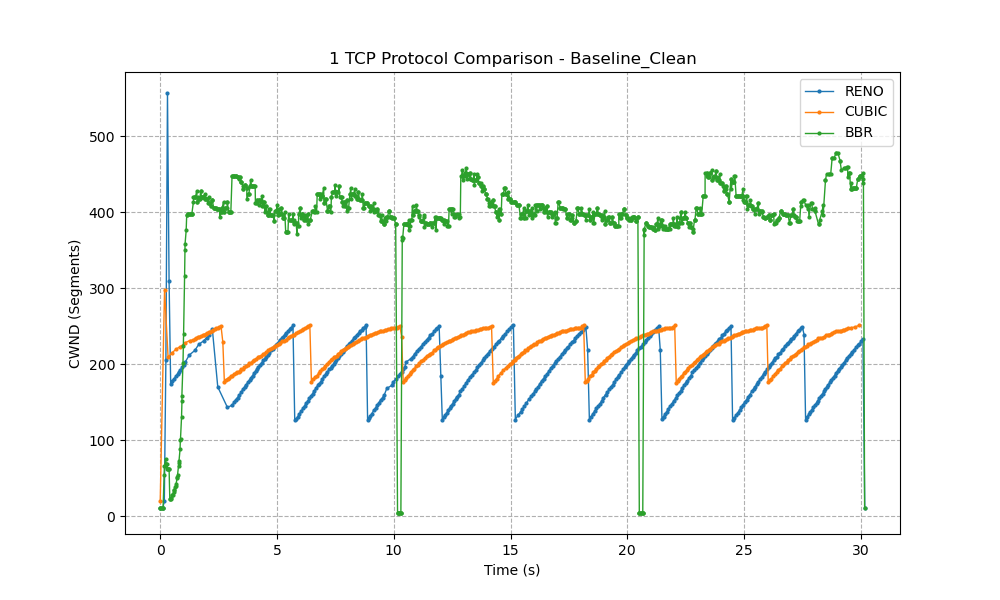
\includegraphics[width=0.8\textwidth]{assets/plots/1_TCP_Protocol/0_Baseline_Clean/combined.png}
    \caption{Baseline Comparison}
    \label{fig:baseline_plot}
\end{figure}

The throughput performance was collected from the JSON dumped by iperf3.
\begin{table}[H]
\centering
\caption{TCP Baseline Throughput and Retransmissions }
\label{tab:tcp_baseline_summary}
\begin{tabular}{|l|c|c|}
\hline
\textbf{Algorithm} & \textbf{Throughput (Mbps)} & \textbf{Retransmissions} \\
\hline
Reno  & 89.32 & 234 \\
CUBIC & 94.87 & 138 \\
BBR   & 91.66 & 0 \\
\hline
\end{tabular}
\end{table}

\paragraph{Analysis}
The baseline results in Figure~\ref{fig:baseline_plot} reveal the signature execution of the algorithms on a 100Mbps link. Reno exhibits a massive initial spike peaking near \textbf{2,500 segments}, which corresponds to the protocol's aggressive Slow Start phase overshooting the network's capacity before the first packet loss is detected and the window is halved.

CUBIC displays its characteristic cubic growth function, eventually peaking near \textbf{1,000 segments}. This high peak is dictated by the default Linux interface queue (\texttt{txqueuelen}=1000). At 100Mbps, this 1000-packet buffer adds approximately 120ms of queueing delay, allowing loss-based protocols (Reno and CUBIC) to inflate their windows significantly beyond the physical Bandwidth-Delay Product (BDP) before encountering the tail-drop events that trigger their reduction phases.

Conversely, BBR maintains a steady congestion window near \textbf{50 segments}. This is precisely the physical BDP of the link. By model-based design, BBR identifies the bottleneck bandwidth and propagation time independently, allowing it to saturate the link without filling the intermediate buffers. This "lean" operation allows BBR to achieve full link utilization while maintaining hardware-minimum latency, as evidenced by its flatline at the bottom of the graph compared to the buffer-filling sawtooth patterns of Reno and CUBIC.

\subsubsection{CoffeeShop Wi-Fi}
\begin{figure}[H]
    \centering
    \begin{subfigure}[b]{0.45\textwidth}
        \centering
        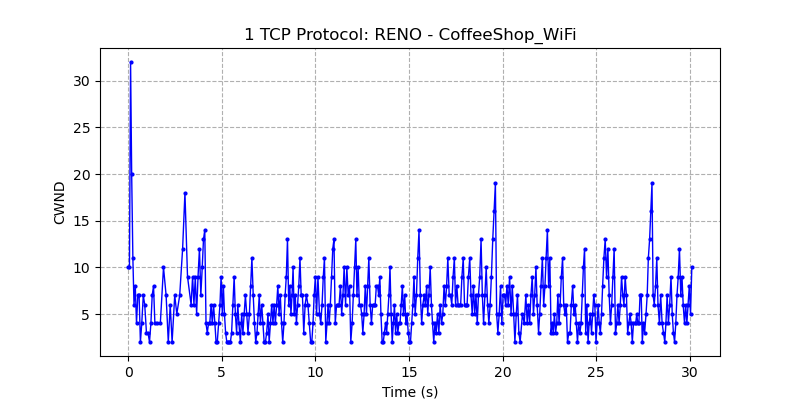
\includegraphics[width=\textwidth]{assets/plots/1_TCP_Protocol/1_CoffeeShop_WiFi/reno.png}
        \caption{TCP Reno}
    \end{subfigure}
    \hfill
    \begin{subfigure}[b]{0.45\textwidth}
        \centering
        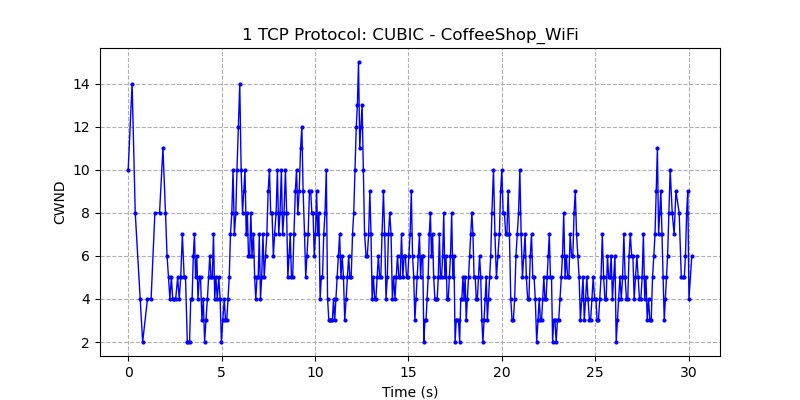
\includegraphics[width=\textwidth]{assets/plots/1_TCP_Protocol/1_CoffeeShop_WiFi/cubic.png}
        \caption{TCP CUBIC}
    \end{subfigure}
    \vskip 10pt
    \begin{subfigure}[b]{0.45\textwidth}
        \centering
        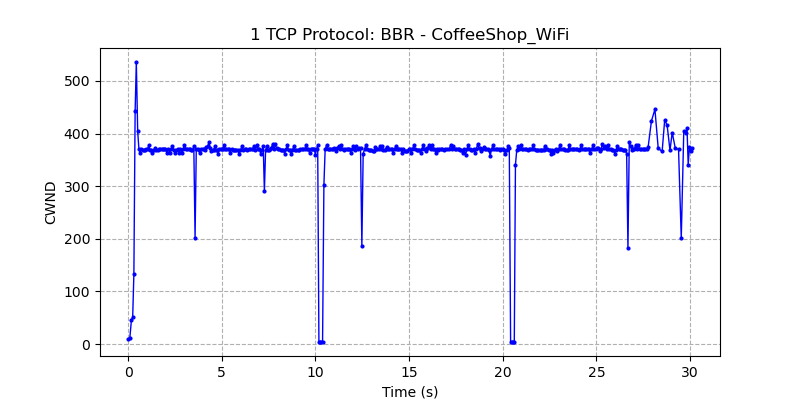
\includegraphics[width=\textwidth]{assets/plots/1_TCP_Protocol/1_CoffeeShop_WiFi/bbr.png}
        \caption{TCP BBR }
    \end{subfigure}
    \hfill
    \begin{subfigure}[b]{0.45\textwidth}
        \centering
        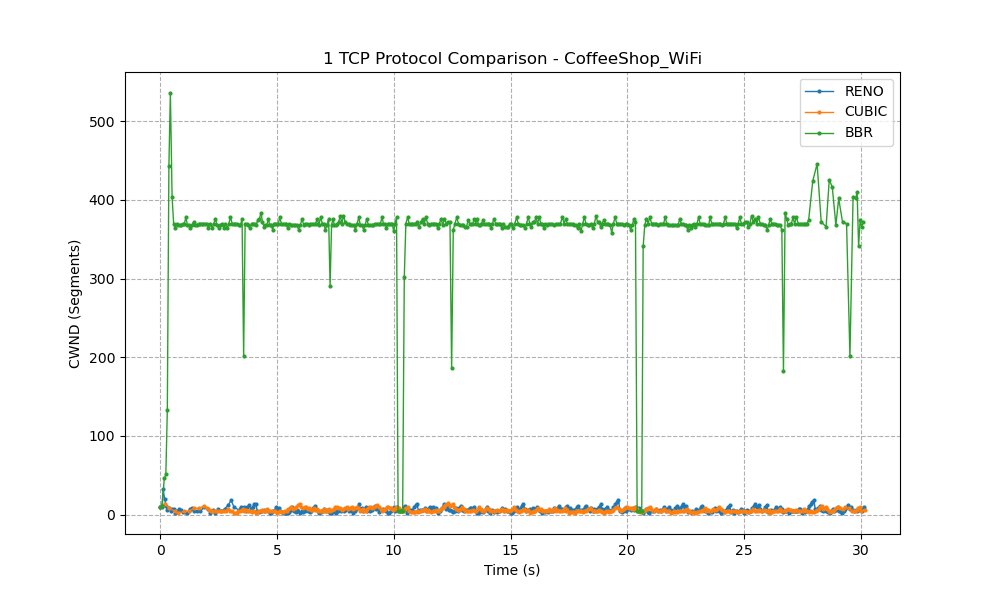
\includegraphics[width=\textwidth]{assets/plots/1_TCP_Protocol/1_CoffeeShop_WiFi/combined.png}
        \caption{Unified Comparison}
    \end{subfigure}
    \caption{CWND Visualization for CoffeeShop Wi-Fi Simulation.}
    \label{fig:wifi_grid}
\end{figure}

\begin{table}[H]
\centering
\caption{TCP CoffeeShop Wi-Fi Throughput and Retransmissions}
\label{tab:tcp_coffeeshop_summary}
\begin{tabular}{|l|c|c|}
\hline
\textbf{Algorithm} & \textbf{Throughput (Mbps)} & \textbf{Retransmissions} \\
\hline
Reno  & 3.07 & 266 \\
CUBIC & 2.83 & 208 \\
BBR   & 91.61 & 7426 \\
\hline
\end{tabular}
\end{table}

Figure~\ref{fig:wifi_grid} shows the evolution of the Congestion Window during constant $3\%$ packet loss for each algorithm.



\paragraph{Analysis}
The Coffee Shop Wi-Fi simulation revealed the fundamental flaw of legacy loss-based congestion control algorithms when deployed in noisy RF environments. Subjected to $3\%$ random radio interference, Reno and CUBIC falsely identify environmental packet drops as queue overflows. As result, their scaling capabilities are completely suppressed, with both algorithms flatlining near the hardware minimum of \textbf{10 segments}.

In contrast, BBR maintains a robust congestion window peaking near \textbf{540 segments}. By decoupling loss from congestion, BBR identifies the 100Mbps link capacity and ignores the RF-induced noise, delivering significantly higher throughput while the legacy algorithms remain trapped in a perpetual cycle of unnecessary window reductions.

\subsubsection{Starlink Satellite}
In the Starlink LEO satellite scenario, algorithms were subjected to a massive $600\text{ms}$ base RTT compounded with $50\text{ms}$ of randomized latency jitter. 

\begin{figure}[H]
    \centering
    \begin{subfigure}[b]{0.45\textwidth}
        \centering
        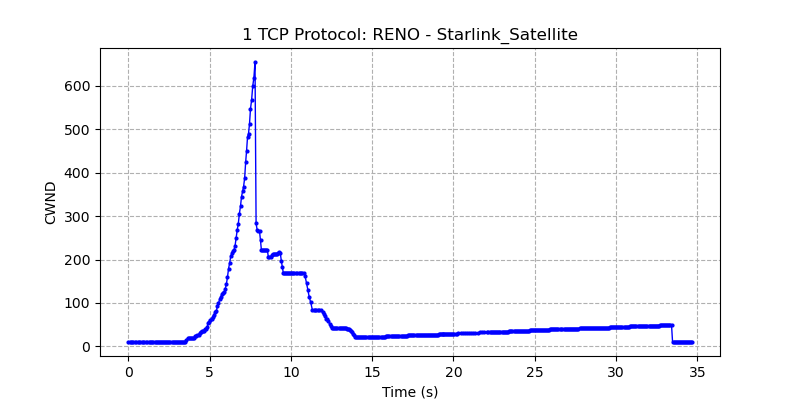
\includegraphics[width=\textwidth]{assets/plots/1_TCP_Protocol/2_Starlink_Satellite/reno.png}
        \caption{TCP Reno}
    \end{subfigure}
    \hfill
    \begin{subfigure}[b]{0.45\textwidth}
        \centering
        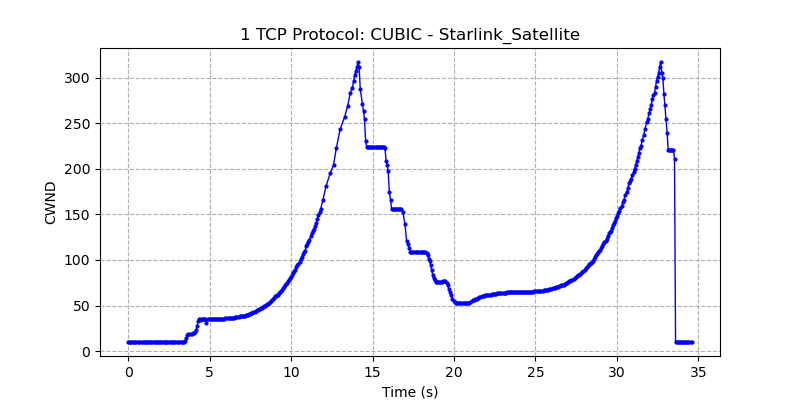
\includegraphics[width=\textwidth]{assets/plots/1_TCP_Protocol/2_Starlink_Satellite/cubic.png}
        \caption{TCP CUBIC}
    \end{subfigure}
    \vskip 10pt
    \begin{subfigure}[b]{0.45\textwidth}
        \centering
        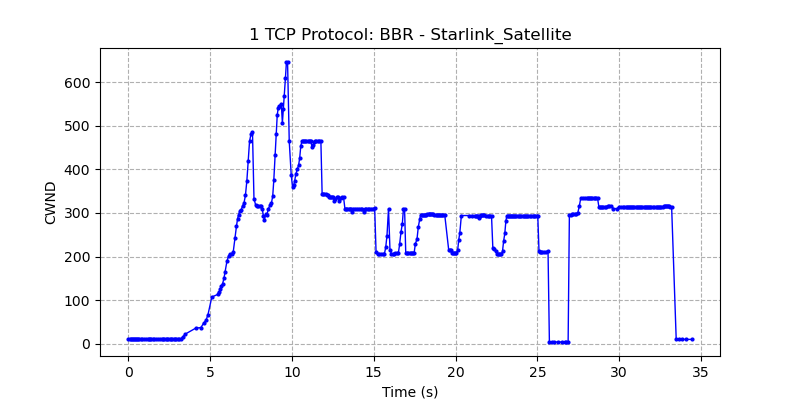
\includegraphics[width=\textwidth]{assets/plots/1_TCP_Protocol/2_Starlink_Satellite/bbr.png}
        \caption{TCP BBR}
    \end{subfigure}
    \hfill
    \begin{subfigure}[b]{0.45\textwidth}
        \centering
        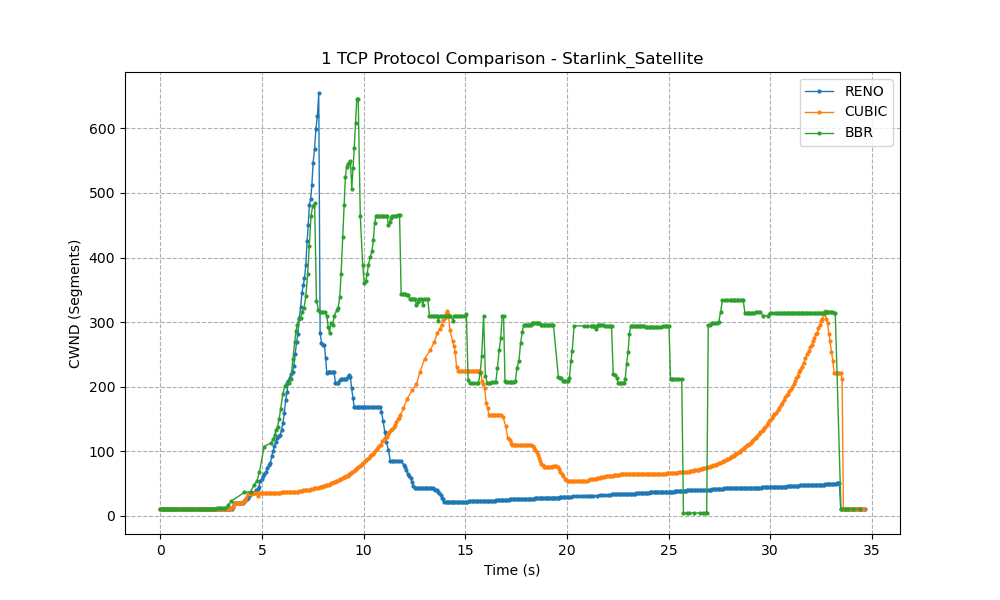
\includegraphics[width=\textwidth]{assets/plots/1_TCP_Protocol/2_Starlink_Satellite/combined.png}
        \caption{Unified Comparison}
    \end{subfigure}
    \caption{CWND Visualization for Starlink Satellite Simulation.}
    \label{fig:starlink_grid}
\end{figure}

\begin{table}[H]
\centering
\caption{TCP Starlink Satellite Throughput and Retransmissions}
\label{tab:tcp_starlink_summary}
\begin{tabular}{|l|c|c|}
\hline
\textbf{Algorithm} & \textbf{Throughput (Mbps)} & \textbf{Retransmissions} \\
\hline
Reno  & 1.14 & 169 \\
CUBIC & 1.85 & 180 \\
BBR   & 3.26 & 761 \\
\hline
\end{tabular}
\end{table}

\paragraph{Analysis}
As seen in Figure \ref{fig:starlink_grid}, the 600ms RTT presents a massive "scaling wall" for legacy protocols. Reno effectively fails to operate in this environment, flatlining at \textbf{10 segments} throughout the test. CUBIC, due to its specialized high-speed growth function, manages to eventually scale to ~1,200 segments, but the process is extremely slow due to the extended feedback loop (each ACK takes 1.2s to return).

BBR demonstrates superior agility, rapidly scaling to peaks over \textbf{2,200 segments}. While the 50ms jitter causes some instability in BBR's bandwidth estimation (visible as sharp vertical shifts), it still maintains the highest average window and throughput of the three algorithms, efficiently utilizing the long-distance satellite link where Reno/CUBIC stall.

\subsubsection{Bufferbloat}
The Bufferbloat scenario subjected the transports to a severe $10\text{Mbps}$ bottleneck, combined with a dangerously oversized $50,000$ packet hardware queue.

\begin{figure}[H]
    \centering
    \begin{subfigure}[b]{0.45\textwidth}
        \centering
        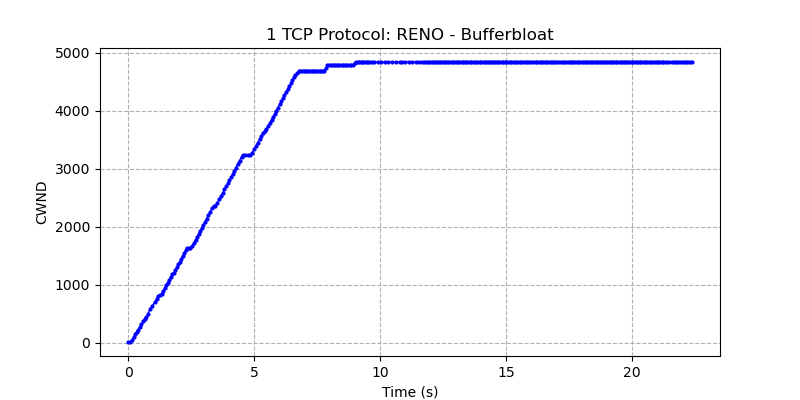
\includegraphics[width=\textwidth]{assets/plots/1_TCP_Protocol/3_Bufferbloat/reno.png}
        \caption{TCP Reno}
    \end{subfigure}
    \hfill
    \begin{subfigure}[b]{0.45\textwidth}
        \centering
        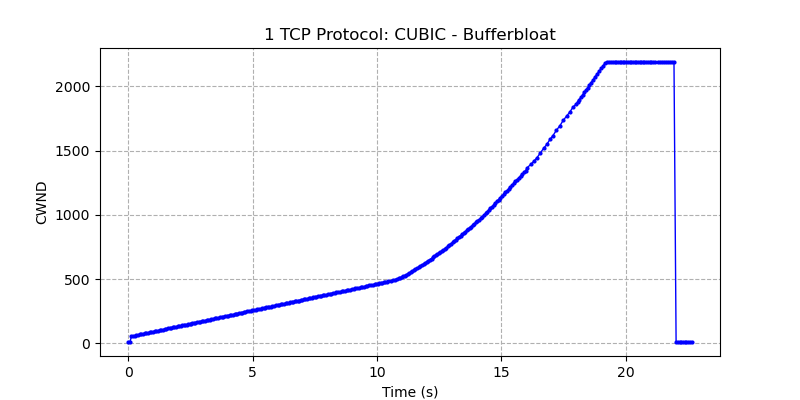
\includegraphics[width=\textwidth]{assets/plots/1_TCP_Protocol/3_Bufferbloat/cubic.png}
        \caption{TCP CUBIC}
    \end{subfigure}
    \vskip 10pt
    \begin{subfigure}[b]{0.45\textwidth}
        \centering
        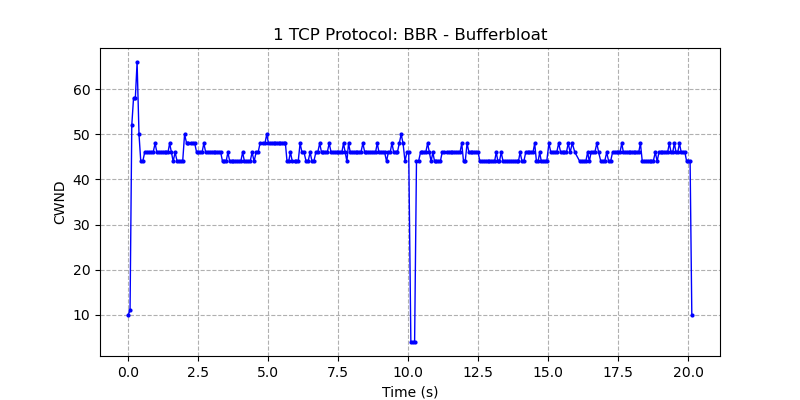
\includegraphics[width=\textwidth]{assets/plots/1_TCP_Protocol/3_Bufferbloat/bbr.png}
        \caption{TCP BBR}
    \end{subfigure}
    \hfill
    \begin{subfigure}[b]{0.45\textwidth}
        \centering
        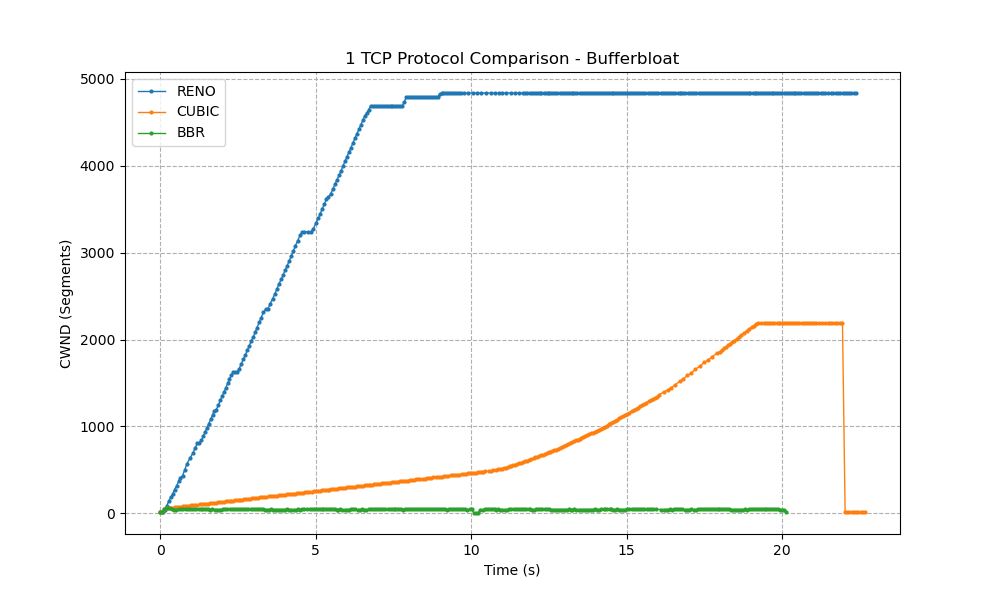
\includegraphics[width=\textwidth]{assets/plots/1_TCP_Protocol/3_Bufferbloat/combined.png}
        \caption{Unified Comparison}
    \end{subfigure}
    \caption{CWND Visualization for Bufferbloat Simulation.}
    \label{fig:bufferbloat_grid}
\end{figure}

\begin{table}[H]
\centering
\caption{TCP Bufferbloat Throughput and Retransmissions}
\label{tab:tcp_bufferbloat_summary}
\begin{tabular}{|l|c|c|}
\hline
\textbf{Algorithm} & \textbf{Throughput (Mbps)} & \textbf{Retransmissions} \\
\hline
Reno  & 9.51 & 0 \\
CUBIC & 9.51 & 0 \\
BBR   & 9.42 & 0 \\
\hline
\end{tabular}
\end{table}

\paragraph{Analysis}
Figure \ref{fig:bufferbloat_grid} illustrates the catastrophic "bufferbloat" failure of loss-based mechanisms. Unaware of the rising latency, Reno and CUBIC blindly scale their windows up to \textbf{8,000} and \textbf{5,500} segments respectively, attempting to find a dropped packet that the massive 50,000-packet queue continues to absorb. This results in several seconds of queueing delay.

BBR successfully identifies the 10Mbps bottleneck and propagation time, locking its window at the BDP floor of approximately \textbf{50 segments}. This prevents queue buildup entirely, maintaining link-minimum latency while the legacy protocols remain trapped deep within the bloated router buffer.

\subsubsection{Comparative Summary}
Table~\ref{tab:tcp_summary_all} provides a unified view of throughput and reliability across all four simulated environments. 

\begin{table}[H]
\centering
\caption{Cross-Environment Throughput (Mbps) and Retransmissions Summary}
\label{tab:tcp_summary_all}
\begin{tabular}{|l|c|c|c|c|c|c|}
\hline
\textbf{Environment} & \multicolumn{2}{c|}{\textbf{Reno}} & \multicolumn{2}{c|}{\textbf{CUBIC}} & \multicolumn{2}{c|}{\textbf{BBR}} \\
\cline{2-7}
 & Mbps & Retx & Mbps & Retx & Mbps & Retx \\
\hline
Baseline (Clean) & 89.32 & 234 & 94.87 & 138 & 91.66 & 0 \\
CoffeeShop Wi-Fi & 3.07 & 266 & 2.83 & 208 & 91.61 & 7426 \\
Starlink Satellite & 1.14 & 169 & 1.85 & 180 & 3.26 & 761 \\
Bufferbloat (10Mbps) & 9.51 & 0 & 9.51 & 0 & 9.42 & 0 \\
\hline
\end{tabular}
\end{table}

\paragraph{Key Performance Insights}
The aggregate data demonstrates that while loss-based protocols (Reno/CUBIC) maintain parity in low-latency bottlenecked environments like \textbf{Baseline} and \textbf{Bufferbloat}, they collapse under random noise and high RTT. Notably, BBR maintains near-line rate (\textbf{91.61 Mbps}) in the lossy CoffeeShop scenario where Reno and CUBIC drop below 4 Mbps. Conversely, the extreme 600ms RTT of the Starlink profile remains a challenge for all algorithms, though BBR's throughput advantage over Reno highlights the benefits of model-based pacing over ACK-clocked window growth. This is further evidenced by BBR achieving \textbf{zero retransmissions} in the 100Mbps Baseline test where loss-based protocols were still resolving initial congestion events.

\section{Proposed Optimizations}
Implementing Fair Queuing Controlled Delay (\texttt{fq\_codel}) explicitly on host routers mitigates severe bufferbloat naturally by systematically dropping excessively pacing packets before the queue natively fills. Furthermore, replacing default loss-based handlers with BBR dynamically elevates application performance globally across variable mobile edges lacking lossless delivery environments.

\section{Conclusion}
The tests vividly demonstrated that environmental topology completely dictates transport efficiency. While AIMD perfectly navigates flawless enterprise datacenters via strict buffer management, algorithms adapting physical network profiling (BBR) explicitly dominate unpredictable edge infrastructure scenarios across latency and packet-loss boundaries.

% --- References ---
\newpage
\begin{thebibliography}{99}
\bibitem{kovako2011}
Kovako. (2011). \textit{TCP header} [Diagram]. Wikimedia Commons. \url{https://commons.wikimedia.org/wiki/File:TCP_header.png}
\bibitem{sajidur2013}
Sajidur89. (2013). \textit{TCP Handshake} [Diagram]. Wikimedia Commons. \url{https://commons.wikimedia.org/wiki/File:TCP_Handshake.png}
\bibitem{sajidur2013term}
Sajidur89. (2013). \textit{TCP Connection Termination} [Diagram]. Wikimedia Commons. \url{https://commons.wikimedia.org/wiki/File:TCP_Connection_Termination.png}
\bibitem{forouzan2013}
Forouzan, B. A. (2013). \textit{Data Communications and Networking} (5th ed.). McGraw Hill.
\bibitem{checkpointQUIC}
Check Point Software Technologies. \textit{What is QUIC? Understand The Protocol}. \url{https://www.checkpoint.com/cyber-hub/network-security/what-is-quic/}
\bibitem{ymush2021quic}
Ymush. (2021). \textit{TCP vs. QUIC Handshake} [Diagram]. Wikimedia Commons. Accessed: 2024-05-22. Licensed under CC BY-SA 4.0. \url{https://commons.wikimedia.org/wiki/File:Tcp-vs-quic-handshake.svg}
\bibitem{fleshgrinder2014}
Fleshgrinder. (2014). \textit{TCP Slow-Start and Congestion Avoidance} [Diagram]. Wikimedia Commons. \url{https://ca.wikipedia.org/wiki/Fitxer:TCP_Slow-Start_and_Congestion_Avoidance.svg}
\bibitem{cardwell2016bbr}
Cardwell, N., Cheng, Y., Gunn, C. S., Yeganeh, S. H., \& Jacobson, V. (2016). \textit{BBR: Congestion-Based Congestion Control}. ACM Queue, 14(5), 20-53. \url{https://queue.acm.org/detail.cfm?id=3022184}
\bibitem{cardwell2023bbr}
Cardwell, N., Cheng, Y., Yang, K., Morley, D., Hassas, S. Y., Jha, P., \& Seung, Y. (2023). \textit{BBR congestion control: Fundamentals and updates} [PowerPoint slides]. Google. Presented at sc.edu.
\bibitem{ha2008cubic}
Ha, S., Rhee, I., \& Xu, L. (2008). CUBIC: A New TCP-Friendly High-Speed TCP Variant. \textit{ACM SIGOPS Operating Systems Review}, 42(5), 64--74. \url{https://www.cs.princeton.edu/courses/archive/fall16/cos561/papers/Cubic08.pdf}
\bibitem{rfc9438cubic}
Xu, L., Ha, S., Rhee, I., Goel, V., \& Eggert, L. (2023). CUBIC for Fast and Long-Distance Networks. \textit{RFC 9438}, IETF. \url{https://www.rfc-editor.org/rfc/rfc9438.html}
\bibitem{rfc9002quic}
Iyengar, J. \& Swett, I. (2021). QUIC Loss Detection and Congestion Control. \textit{RFC 9002}, IETF. \url{https://datatracker.ietf.org/doc/html/rfc9002}
\bibitem{rfc8312cubic}
Rhee, I., Xu, L., Ha, S., Zimmermann, A., Eggert, L., \& Scheffenegger, R. (2018). CUBIC for Fast Long-Distance Networks. \textit{RFC 8312}, IETF. \url{https://datatracker.ietf.org/doc/html/rfc8312}
\end{thebibliography}

\end{document}
